%
%
%

\documentclass[journal=jctcce,manuscript=suppinfo]{achemso}

\usepackage[T1]{fontenc}
\usepackage{graphicx}
\usepackage{amsmath}
\usepackage{amssymb}
\usepackage{xcolor}


\title{Reproducing Relative Alchemical Free Energies of Hydration}

\author{Hannes H. Loeffler}
\affiliation[Scientific Computing Department, STFC]{Science \&
  Technology Facilities Council, Daresbury, Warrington, WA4 4AD,
  United Kingdom}
\email{Hannes.Loeffler@stfc.ac.uk} \phone{+44 1925 603367}

\author{Stefano Bosisio}
\affiliation[University of Edinburgh]{EaStCHEM School of Chemistry,
  University of Edinburgh, David Brewster Road, Edinburgh EH9 3FJ, UK}

\author{Guilherme Duarte Ramos Matos}
\affiliation[University of California, Irvine]{Department of
  Chemistry, University of California, Irvine}

\author{Donghyuk Suh}
\affiliation[University of Chicago]{University of Chicago}

\author{Julien Michel}
\affiliation[University of Edinburgh]{EaStCHEM School of Chemistry,
  University of Edinburgh, David Brewster Road, Edinburgh EH9 3FJ, UK}

\author{David L. Mobley}
\affiliation[University of California, Irvine]{Departments of
  Pharmaceutical Sciences and Chemistry, University of California,
  Irvine}

\author{Benoit Roux}
\affiliation[University of Chicago]{University of Chicago}


\keywords{Free Energy, Hydration, Alchemical, Reproducibility}


\begin{document}

\maketitle

% whole table comparing all softwares used in the study
% input files (coordinates and topologies)
% lambda schedules used in the simulations (mdp files?)
% glossary: what do terms used in the main text mean
% . alternatives used by other workers (lots of work! -> worthwhile?)


\section{Softcore Functions}

We describe here the softcore functions~\cite{beutler_avoiding_1994,
  zacharias_separationshifted_1994} as implemented in the MD packages
AMBER, CHARMM, Gromacs and Sire.  Both the van der Waals,
$V_{\mathrm{LJ}}$ (Lennard--Jones potential) and the electrostatic
interactions, $V_{\mathrm{Coul}}$ (Coulomb potential) as a function of
the order parameter $\lambda$ are given for the disappearing atoms
only.  For the appearing atoms replace $\lambda$ with $1 - \lambda$
and \emph{vice versa}.  Eq.\ \eqref{eq:general} is the generalized
form for all codes while the specific distance dependent functions are
outlined in eq.\,\eqref{eq:Sire} for Sire, eq.\,\eqref{eq:Amber} for
AMBER, eq.\,\eqref{eq:Gromacs} for Gromacs and eq.\,\eqref{eq:CHARMM}
for CHARMM.

\begin{equation}
  V = V_{\mathrm{LJ}} + V_{\mathrm{Coul}} =
  4\epsilon_{\mathrm{ij}}(1 - \lambda) \left[ \left(
      \frac{\sigma_{ij}}{\textcolor{red}{r_{\mathrm{LJ}}}}
    \right)^{12} - \left(
      \frac{\sigma_{ij}}{\textcolor{red}{r_{\mathrm{LJ}}}} \right)^{
      6} \right] +
  (1 - \lambda)^{n} \frac{q_{i}q_{j}}
  {4\pi\varepsilon_{0}\textcolor{red}{r_{\mathrm{Coul}}}}
  \label{eq:general}
\end{equation}

For Sire
\begin{equation}
  \begin{split}
    r_{\mathrm{LJ}} &= (\alpha\sigma_{ij}\lambda + r_{ij}^2)^{\frac{1}{2}} \\
    r_{\mathrm{Coul}} &=  (\lambda + r_{ij}^2)^{\frac{1}{2}}
  \end{split}
  \label{eq:Sire}
\end{equation}

For AMBER
\begin{equation}
  \begin{split}
    r_{\mathrm{LJ}} &= (\alpha \sigma_{ij}^{6} \lambda + % see JCP127, 214108
                         r_{ij}^6)^{\frac{1}{6}} \\
    r_{\mathrm{Coul}} &= (\beta\lambda + r_{ij}^{p})^{\frac{1}{p}} \\
    n &= 1
  \end{split}
  \label{eq:Amber}
\end{equation}

For Gromacs
\begin{equation}
  \begin{split}
    r_{\mathrm{LJ}} &= (\alpha \sigma_{ij}^{w} \lambda^{p} +
    r_{ij}^{w})^{\frac{1}{w}} \\
    &p = 1,2; w = 6,48; \\
    r_{\mathrm{Coul}} &= r_{\mathrm{LJ}} \\
    &\alpha_{\mathrm{Coul}} = 0,\alpha_{\mathrm{LJ}} \\
    n &= 1
  \end{split}
  \label{eq:Gromacs}
\end{equation}

For CHARMM (PSSP), applied to all ``reactant'' and all ``product'' atoms
\begin{equation}
  \begin{split}
    r_{\mathrm{LJ}} &= (\alpha \lambda + r_{ij}^2)^{\frac{1}{2}} \\
    r_{\mathrm{Coul}} &= (\beta\lambda + r_{ij}^{2})^{\frac{1}{2}} \\
    n &= 1
   \end{split}
  \label{eq:CHARMM}
\end{equation}

$r_{\mathrm{vdW}}$ and $r_{\mathrm{Coul}}$ (both in red) are the
distance dependent functions, $\epsilon_{\mathrm{Coul}}$ and
$\sigma_{ij}$ are the Lennard-Jones parameters, $q_{i}$ and $q_{j}$
are the charges and $\varepsilon_{0}$ is the vacuum permittivity,
$\alpha$ and $\beta$ are the softcore tuning parameters determining
the softness of the potential, and $r_{ij}$ the distance between
atoms.

$n$ is an exponent only used in the Coulomb softcore funtion of Sire.
Gromacs allows additional exponents for $\lambda$ ($p = 1$ or $2$) and
$w$ for the distance dependency with values of either $6$ or $48$.
The Coulomb softcore parameter $\alpha_{\mathrm{Coul}}$ in Gromacs is
the same as for the Lennard--Jones parameter $\alpha_{\mathrm{LJ}}$
unless the Coulomb softcore function is requested not to be used.  The
CHARMM softcore function (PSSP) is applied to \emph{all} atoms in the
perturbed group and not only to dummy atoms as in the other codes.
The perturbed group comprises of all atoms that need to be
transformed, i.e.\ any atom that differs in at least one force field
parameter in the other end state.  ``Dummy'' atom is used here as a
shorthand notation for any atom that appears or disappears during the
course of the transformation.


\section{Separated Protocols}

When the AFE (alchemiccal free energy) simulation is separated into van
der Waals and Coulomb steps it must be ensured that charges of
vanishing atoms are switched off before the vdW radius is scaled to
zero.  This is to avoid that other atoms e.g.\ from solvent come in
close contact to a charged atom without the associated excluded volume
from the van der Walls term.

\begin{figure}[ht]
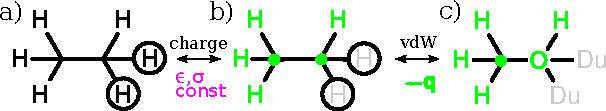
\includegraphics[scale=1.0]{figures/dummies.pdf}
\caption{The mutation of ethane into methanol and explict topologies
  for three states. a) The two circles denote atoms that have both vdW
  and Coulomb terms switched on with parameters for the respective
  hydrogen atom type.  b) The two hydrogen atoms have their charges
  switched to zero (grey symbols in black circle).  All other charges
  are the ones from the methanol end state c (green) to ensures charge
  neutrality at each step.  VdW parameters are constant in the charge
  transfer step (see annotations in magenta).  c) vdW and Coulomb
  parameters as for methanol while dummy atoms (grey Du) have those
  parameters all set to zero.}
\label{fig:dummies}
\end{figure}

Figure~\ref{fig:dummies} depicts how force field parameters vary for a
transformation carried out in the direction of disappearing atoms.
The mutation is shown with the charge step first followed by the vdW
step but each step can really be run independently.  Please note that
both charge and vdW step would be simulated at a range of individual
$\lambda$s.  Typically the charge transfer is done with linear scaling
while the vdW mutation is done with softcores (see above).  The
transformation is fully symmetrical that is the parameters must be
switched on in opposite order if atoms are to be ``created''.  The
intermediate state b has the vdW parameters from state a but the
charges from state c.

Figure~\ref{fig:dummies} shows how topology files may be created in
the case that the MD software does not allow independent $\lambda$s
for electrostatic and vdW mutations.  With Gromacs, for instance, the
transformation only requires a single topology file with both A and B
states (in single topology fashion, see main text) and a single
simulation control file with separate $\lambda$ vectors for charge and
vdW transformations.  Any intermediate state from
Figure~\ref{fig:dummies} is thus created ``on--the-fly'' i.e.\
implictly during the simulation run.  With AMBER (up to version 16 as
of this writing), however, three eplicit topology files (with sander,
two with pmemd) and two control files would need to be created.  The
state b in Figure~\ref{fig:dummies} would be created from state a with
the charges from state c.  The bonded terms can be combined with
either mutation step or run separately.  For AMBER the easiest is to
combine vdW with bonded terms because charges are independent of atom
types.

Figure~\ref{fig:dummies2} illustrates excplicit topologies for
transformations with both appearing and disappearing atoms.  The
principle is essentially the same as in Figure~\ref{fig:dummies}:
charges of dummy atoms must be switched off before vdW parameters are
set to zero to avoid interactions of ``naked'' charge sites with other
atoms possibly leading to very close contact, large energies and
forces, and thus to unstable simulations and/or noisy statistics.
However, charge neutrality at every $\lambda$ step is not supported in
most MD codes i.e.\ the total system charge varies with $\lambda$
unless the charges of \emph{all} atoms are switched off.  Possible
strategies would be to explictly create topology files for each
intermediate $\lambda$ state and distribute the dimished charges from
the dummy atoms over to the non--dummy atoms.  MD software like CHARMM
allow to do this through scripting although this would be just as
extensive as scripting the aforementioned strategy.

\begin{figure}[ht]
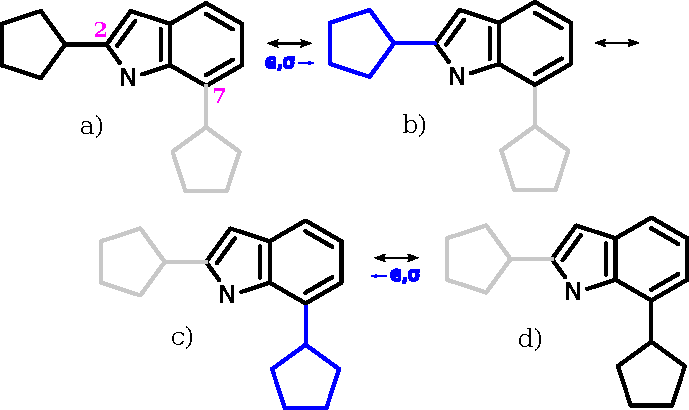
\includegraphics[scale=1.0]{figures/dummies2.pdf}
\caption{Explicit topologies involved in a mutation with both
  appearing and disappearing atoms by example of the cyclopentanyl
  transfer from the 2 position in indole to the 7 position.  Green
  lines denote atoms which have their charges switched off but with
  vdW parameters from the left (state b) or right (state c). Grey
  lines are dummy atoms with Coulomb and vdW parameters all zero.
  Note, the hydrogen bound to the 2 (state d) and 7 positions (state
  a) can be directly mutated from the respective carbon atom type
  without ring breaking~\cite{doi:10.1021/acs.jcim.5b00057}.}
\label{fig:dummies2}
\end{figure}

With the MD packages tested in this study the number of input files
are as follows.  With Gromacs this can be done with only two topology
and two control files where one charge transfer can be combined with a
vdW on/off step.  Gromacs' $\lambda$ vectors only apply to the
perturbed group as a whole and so it is not possible to define a
$\lambda$ vector for only a subset.  AMBER requires two such files
with sander and three topology/two control files with pmemd for the
steps charge off, vdw on/off and charge on.  This is possible because
with AMBER a subset of the perturbed group can be chosen to have zero
charges (but AMBER does not have $\lambda$ vectors).  CHARMM has
scripting facilities that let the user manipulate force field
parameters of any arbitrary subset of the system such that
intermediate states can be defined ``on--the-fly'' with only one
control script and one topology file.  The tool
FESetup~\cite{loeffler_fesetup:_2015} automates most of these setup
steps.

\bibliography{journal-abbrev,reprod}

\end{document}
